\chapter{Pricing Theories}

\section{Credit Derivative Approach} \label{sec:creditderivativeapproach}

In financial markets the reduced-form approach is widely used in order to price credit risk. It was originally introduced by \citet{jarrow1995pricing} respectively \citet{duffie1999modeling}. The credit derivative approach applies the reduced-form approach to CoCos. In this context, the derivation of a pricing formula for CoCos follows mainly \citet{de2011pricing}. 

\subsection{Reduced-Form Approach and Credit Triangle}

The reduced-form approach is an elegant way of bridging the gap between the prediction of default and the pricing of default risk of a straight bond. In the following, we investigate the link between estimated default intensities and credit spreads under the reduced-form approach. \citep{lando2009credit}\\

Let $\tau$ denote the random time of default of some company. It is assumed that the distribution of $\tau$ has a continuous density function $f$, so that the distribution function $F$ and the curve of survival probabilities $q$ are related as follows:  
\begin{align}
P(\tau \leq t) &= F(t) = 1 - q(t) = \int_0^t f(s) ds \text{, with } t \geq 0
\end{align}

The hazard rate respectively the default intensity $\lambda$ is defined as follows:
\begin{align} \label{hazardrate}
\lambda(t) &= \lim_{\Delta \downarrow 0} \dfrac{1}{\Delta} P(\tau \leq t + \Delta | \tau > t) = \dfrac{F'(t)}{q(t)} = \dfrac{F'(t)}{1 - F(t)} = - \dfrac{d}{dt} \log q(t)
\end{align}
Intuitively, the hazard rate is the default rate per year as of today. Using \ref{hazardrate} we can derive a formula for the survival probability:
\begin{align}
q(t) &= \exp \left(- \int_0^t \lambda (s) ds \right)
\end{align}

For our application of the reduced-form approach we assume that the hazard rate $\lambda(t)$ is a deterministic function of time. In reality $\lambda(t)$ is not deterministic but itself stochastic. That fits in with the fact that credit spreads are not static but stochastically varying over time. \citep{lectureschmidt} However, we further consider the hazard rate to be constant in order to simplify the problem. Hence, a constant hazard rate $\lambda(t) = \lambda$ implies an exponential distribution of the default time:
\begin{align} \label{bonddefaultprob}
F(t) &=  1 - q(t) = 1 - \exp (- \lambda t)
\end{align}

Under the idealized assumption of a flat zero interest rate curve, a flat spread curve and continuous spread payments, the default intensity $\lambda$ can be calculated directly from the credit spread $s$ and the recovery rate $R$ by the rule of thumb formula \citep{lectureschmidt}, which is also known as credit triangle: 
\begin{align}
\lambda &= \dfrac{s}{1 - R}
\end{align}
Finally, this relationship makes it possible to determine the default probability $F$ from the credit spread $s$ and vice versa.

\subsection{Adaption to CoCos}
In accordance with the aforementioned reduced-form approach, \citet{de2011pricing} assume that the probability $F^*$, which measures the likelihood that a CoCo triggers within the next $T - t$ years, follows similar mechanics as the default probability of a straight bond does. Under the credit derivative approach the probability $F^*$ can be expressed as follows:
\begin{align} \label{cocodefaultprob}
    F^* &= 1 - \exp\left[- \lambda_{Trigger} (T-t)\right]
\end{align}

Additionally, the credit derivative approach models $F^*$ with the first exit time equation used in barrier option pricing under a Black-Scholes setting. \citep{su2009likely} Hence, the probability $F^*$ that the trigger level $S^*$ is touched within the next $T - t$ years is given by the following equation with the continuous dividend yield $q$, the continuous interest rate $r$, the drift $\mu$, the volatility $\sigma$ and the current share price $S$ of the issuing company: 
\begin{align}
    F^* = \Phi\left( \dfrac{\log \left(\dfrac{S^*}{S}\right) - \mu (T - t)}{\sigma \sqrt{(T - t)}}\right) + \left(\dfrac{S^*}{S}\right)^{\dfrac{2 \mu}{\sigma^2}} \Phi\left( \dfrac{\log \left(\dfrac{S^*}{S}\right) + \mu (T - t)}{\sigma \sqrt{(T - t)}}\right)
\end{align}

In this regard, a CoCo's credit spread $s_{CoCo}$ can be approximated by the credit triangle, where $R_{CoCo}$ denotes the recovery rate of a CoCo and $L_{CoCo}$ is the loss rate:
\begin{align} \label{cocospread}
    s_{CoCo} &= \left(1 - R_{CoCo}\right) \lambda_{Trigger} = {L}_{CoCo} \lambda_{Trigger}
\end{align}

In the trigger event, the face value $N$ converts into $C_r$ shares worth $S^*$. The loss of a long position in a CoCo is therefore determined by the conversion price $C_p$:
\begin{align} \label{cocoloss}
    {Loss}_{CoCo} &= N - C_r S^* = N \left(1 - R_{CoCo} \right) = N \left(1 - \dfrac{S^*}{C_p} \right)
\end{align} 

By combining \ref{cocodefaultprob}, \ref{cocospread} and \ref{cocoloss} we see that the credit spread $s_{CoCo}$ of a CoCo with maturity $T$ at time $t$ is driven by its major design elements, the trigger level $S^*$ and the conversion price $C_p$:
\begin{align}
s_{CoCo_t}&= - \dfrac{\log (1 - F^*)}{(T - t)} \left( 1 - \dfrac{S^*}{C_p} \right)
\end{align}

Subsequently, a pricing formula for CoCos under the credit derivative approach can be derived. The present value $V^{cd}$ at time t is given by:
\begin{align}
V^{cd}_t &= \sum^T_{i=1} c_i \exp\left[-(r + s_{CoCo_t}) (t_i - t)\right] + N \exp\left[-(r+s_{CoCo_t}) (T-t) \right]
\end{align}

In summary, the credit derivative approach provides us with a concise method to price CoCos. However, one has to bear in mind its largest shortcoming. Losses from cancelled coupons of triggered CoCos are not taken into account in the valuation. Hence, the credit derivative approach naturally overestimates the price of CoCos, but it equips investors with a simple rule of thumb formula. 

\subsection{Parameter Classification and Adjustment} \label{creditparameterssection}
The credit derivative approach requires several model inputs which can be found in table \ref{creditparameters}. Generally, one can separate three different types. Static inputs comprise parameters that are specified ex ante and are assumed to be constant. Dynamic inputs are updated regularly. Fitting parameters are used to fit the model prices to market prices. \citep{wilkens2014contingent}

\begin{table}[H]
	\setlength{\extrarowheight}{2.5pt}
	\centering
	\begin{tabular}{llll}
		\toprule
			 & \textbf{Description} & \textbf{Usage} & \textbf{Source} \\
		\midrule
			$T$ & Maturity & Static input & Term sheet \\
			$N$ & Notional & Static input & Term sheet \\			
			$c$ & Coupon rate & Static input & Term sheet \\
			$S_0$ & Initial share price & Dynamic input & Market data \\
			$S^*$ & Trigger share price & Fitting parameter & -- \\
			$C_p$ & Conversion price & Static input & Term sheet \\
			$r$ & Risk-free interest rate & Dynamic input & Market data \\
			$q$ & Dividend yield & Dynamic input & Market data\\
			$\sigma$& Share price volatility & Dynamic input & Market data \\
		\bottomrule
	\end{tabular}
	\caption[Parameter classification of the credit derivative approach]{Parameter classification of the credit derivative approach \citep{wilkens2014contingent}}
	\label{creditparameters}
\end{table}

All static inputs can be found in the term sheets of the respective CoCo. But beyond the model depends upon further dynamic inputs among others the share price $S$, the risk-free interest rate $r$, the dividend yield $q$ and the share price volatility $\sigma$. The daily share price $S$ is directly observed in the market. The risk-free interest rate $r$ is derived from sovereign bonds with the same maturity and currency. Furthermore, the input parameter $q$ relies on the three year average dividend yield of the issuing company. The share price volatility $\sigma$ is derived based on a yearly average volatility on a reference stock market index of the last five years similar to \citet{alvemar2012modelling}. In addition, the only degree of freedom in the credit derivative approach is the fitting parameter $S^*$ respectively the trigger share price. Because this input variable is neither a static parameter nor a market parameter, $S^*$ is adjusted by minimizing the root mean squared deviation to realized CoCo prices. \citep{erismann2011analytical}

\subsection{Model Application}

In the following a fictive CoCo is priced with the credit derivative approach pursuantly the specifications as stated in table \ref{creditcoco}. After installing both R, a programming language for statistical computing, and Rstudio, an open-source integrated development environment, a reader can easily price the aforementioned CoCo example with the source code of chapter \ref{creditderivativeapproach}. The CoCo specifications are also used to analyze the price sensitivity in regard to certain input parameters. The results of the sensitivity analysis for the credit derivative approach can be found in section \ref{sensicredit}. In addition, this example data set is also used to apply the equity derivative approach and the structural approach.

\begin{table}[H]
	\setlength{\extrarowheight}{2.5pt}
	\centering
	\begin{tabular}{lrl}
		\toprule
			 & \textbf{Value} & \textbf{Comment} \\
		\midrule
			$T$ & $10$yrs & Maturity \\
			$N$ & $100\%$ & Nominal \\			
			$c$ & $6.00\%$ & Coupon rate \\
			$S_0$ & $120$ & Initial share price\\
			$S^*$ & $60$ & Trigger share price \\
			$C_p$ & $75$ & Conversion price \\
			$r$ & $3.00 \%$ & Risk-free interest rate\\
			$q$ & $0.00\%$ & Dividend yield \\
			$\sigma_E$ & $30.00\%$ & Share price volatility \\
		\bottomrule
	\end{tabular}
	\caption[Parameter specification of credit derivative approach application]{Parameter specification of credit derivative approach application \citep{alvemar2012modelling}}
	\label{creditcoco}
\end{table}

The spread of the CoCo $s_{CoCo}$, which compensates an investor for the risk of equity conversion, equals $1.46\%$. Moreover,  the price $V^{cd}$ of the fictive CoCo under the credit derivative approach equates to $111.31$.

\section{Equity Derivative Approach} \label{sec:equityderivativeapproach}

In order to assess the value of a CoCo, investors can use a method which depends on equity derivatives. \citep{de2011pricing, de2014handbook} The so-called equity derivative approach attempts to compensate for the main drawback of the credit derivative approach, since it takes into account that coupon payments might be cancelled if the trigger of a CoCo was touched.\\

Subsequently, the valuation can be divided into two steps: In the first step, the value of a CoCo is determined without coupon payments. Such a CoCo is called Zero-Coupon CoCo. In the second step, one has to incorporate the coupon payments in the pricing formula while keeping in mind that they might be knocked out. The closed-form solution is derived under a Black-Scholes setting.

\subsection{Step One - Zero-Coupon CoCo}

To determine the present value of a Zero-Coupon CoCo $V^{zcoco}$ at maturity $T$ we can use equation \ref{valueatmaturity}. The underlying assumption of the equity derivative approach is that the triggering of a CoCo respectively of a Zero-Coupon CoCo is equivalent to the share price falling below the level $S^*$. %The indicator function $\mathbbm{1}_{\{ \tau \leq T \}}$ equals one when trigger is touched at the time $\tau$, whereby $\tau$ is element of $[\tau, T]$.
\begin{align} \label{pvedcoco}    
    V^{zcoco}_T &= \begin{cases} N & \text{if not triggered}\\ (1 - \alpha) N + \frac{\alpha N}{C_p} S^{*} & \text{if triggered} \end{cases} \nonumber\\
    &= N \mathbbm{1}_{\{ \tau > T \}} +\left[ \left( 1 - \alpha \right) N + \dfrac{\alpha N}{C_p } S^* \right] \mathbbm{1}_{\{ \tau \leq T \}}\nonumber\\
    &= N + \left[ \dfrac{\alpha N}{C_p} S^* - \alpha N \right] \mathbbm{1}_{\{ \tau \leq T \}}\nonumber\\
    &= N + \left[ C_r S^* - \alpha N \right] \mathbbm{1}_{\{ \tau \leq T \}}\nonumber\\
    &= N + C_r \left[S^* - \dfrac{\alpha N}{C_r}\right] \mathbbm{1}_{\{ \tau \leq T \}}\nonumber\\
    &= N + C_r \left[ S^* - C_p \right] \mathbbm{1}_{\{ \tau \leq T \}}
\end{align}

It may be inferred that the financial payoff of equation \ref{pvedcoco} consists of two components \citep{erismann2015pricing}: (1) the face value $N$ of a zero bond and (2) a long position in $C_r$ shares generating a payoff only if the CoCo materializes at time $\tau$. This component can be approximated with a knock-in forward. The intuition behind equation \ref{pvedcoco} is that if the share price falls below a certain level $S^*$, an investor will use the face value $N$ to exercise the knock-in forward. That said, the investor is committed to buy the amount of $C_r$ shares for the price of $C_p$ at maturity $T$.\\

Before maturity the present value of a Zero-Coupon CoCo $V^{zcoco}$ can be determined by adding up the present value of a zero bond $V^{zb}$ and the present value of a knock-in forward $V_t^{kifwd}$. Hereinafter, the components will be explained briefly. 
\begin{align} \label{pvzcoco}
V^{zcoco}_t &= V^{zb}_t + V_t^{kifwd}
\end{align}

with
\begin{align} 
V^{zb}_t &= N \exp\left[- r (T - t)\right]
\end{align}

Moreover, the long position in shares at time $t$ can be approximated with the respective closed-form solution of a knock-in forward. \citep{hull2006options} 
\begin{align}
    V_t^{kifwd} &= C_r \left[ S_t \exp\left[- q \left(T-t\right)\right]\left(\dfrac{S^*}{S_t}\right)^{2 \lambda} \Phi\left(y_1\right) \right.\nonumber\\
   &\qquad \left.\vphantom{\dfrac{S^*}{S_t}} - K \exp\left[- r \left(T-t\right)\right] \left(\dfrac{S^*}{S_t}\right)^{2 \lambda - 2} \Phi\left(y_1 - \sigma \sqrt{T-t}\right) \right.\nonumber\\
   &\qquad \left.\vphantom{\dfrac{S^*}{S_t}} - K \exp\left[- r \left(T-t\right)\right] \Phi\left(-x_1 - \sigma \sqrt{T-t}\right) \right.\nonumber\\
   &\qquad \left.\vphantom{\dfrac{S^*}{S_t}} + S_t \exp\left[- q \left(T-t\right)\right] \Phi\left(- x_1\right) \right] 
\end{align}

with 
\begin{align*}
C_r &= \dfrac{\alpha N}{C_p}\\
K &= C_p\\
\lambda &= \dfrac{r-q+\dfrac{\sigma^2}{2}}{\sigma^2}\\
x_1 &= \dfrac{\log\left(\dfrac{S_t}{S^*} \right)}{\sigma \sqrt{T-t}} + \lambda \sigma \sqrt{T-t}\\
y_1 &= \dfrac{\log\left(\dfrac{S^*}{S_t} \right)}{\sigma \sqrt{T-t}} + \lambda \sigma \sqrt{T-t}\\
\end{align*}


%
\begin{comment}
A knock-in forward consists of a long position in a knock-in call and a short position in a knock-in put on the underlying shares both with strike K which is equal to the conversion price $C_p$ and with the barrier level being equal to trigger price $S^*$.


\begin{itemize}
\item closed form solution exists for both knock-in options \citep{merton1973theory}
\item price of knock-in call $V^{kic}$ and knock-in put $V^{kip}$ at time $t$ can be calculated with:
\end{itemize}

\begin{align} \label{pvkic}
V_t^{ kic } &= S_t \exp \left[ - q \left(T-t\right) \right] \left( \dfrac{ S^* }{ S_t } \right) ^ { 2 \lambda } \Phi\left( y \right)\nonumber \\ 
&- K \exp \left[ - r \left(T-t\right) \right] \left( \dfrac{ S^* }{ S_t } \right) ^ { 2 \lambda - 2} \Phi \left( y - \sigma \sqrt{T-t} \right)
\end{align}

with 

\begin{align*}
K &= C_p\\
y &= \dfrac{\log\left( \dfrac{S^{* 2}}{S_t K} \right)}{\sigma \sqrt{T-t}} + \lambda \sigma \sqrt{T-t}\\
\lambda &= \dfrac{r-q+\dfrac{\sigma^2}{2}}{\sigma^2}
\end{align*}

\begin{align} \label{pvkip}
V_t^{kip} &=  S_t \exp\left[ -q\left(T-t\right) \right] \left( \dfrac{S^*}{S_t} \right)^{2\lambda} \left[ \Phi\left(y\right) - \Phi\left(y_1 \right) \right]\nonumber\\
&- K \exp\left[ -r\left(T-t\right) \right] \left(\dfrac{S^*}{S_t}\right)^{2\lambda-2}\left[ \Phi\left( y- \sigma \sqrt{T-t} \right) -\Phi \left( y_1 - \sigma \sqrt{T} \right) \right] \nonumber\\
&+ K \exp\left[ - r \left(T-t\right) \right] \Phi \left( x_1 + \sigma \sqrt{T-t} \right)\nonumber\\
 &-S_t \exp\left[ -q \left(T-t\right) \right] \Phi\left( -x_1 \right)
\end{align}

with

\begin{align*}
x_1 &= \dfrac{\log\left(\dfrac{S_t}{S^*} \right)}{\sigma \sqrt{T-t}} + \lambda \sigma \sqrt{T-t}\\
y_1 &= \dfrac{\log\left(\dfrac{S^*}{S_t} \right)}{\sigma \sqrt{T-t}} + \lambda \sigma \sqrt{T-t}
\end{align*}

\begin{itemize}
\item knock-in forward can be constructed with knock-in call and knock-in put \citep{hull2006options}
\item hence, price of knock-in forward $V^{ kifwd }$ at time $t$ can be replicated using equation \ref{pvkic} and \ref{pvkip}:
\end{itemize}
\end{comment}
%

It is important, however, to recognize that a subtle difference exists between the actual economic payoff of equation \ref{pvedcoco} and its replication with a knock-in forward, since the knock-in forward replicates an economic ownership of shares at maturity $T$. Though, the triggering of a CoCo forces investors to accept the conversion immediately. This could lead to an economic ownership of shares at trigger time $\tau$ and, thus, prior to $T$. Therefore, one could argue that receiving a knock-in forward in the trigger event disregards the dividends which a shareholder would receive in particular when a CoCo triggers early. \citet{de2011pricing} argue that dividends can be neglected because distressed banks are likely to behave with great restraint when it comes to dividend payments.

\subsection{Step Two - Adding Coupons}
As mentioned earlier, the first step excludes coupon payments from the valuation. Yet, in this step we want to include them in order to replicate the exact payout profile of a CoCo. Therefore, we replace the zero bond in equation \ref{pvzcoco} with a straight bond with regular coupon payments $c$. Besides, a third component has to be added which takes into account the foregone coupon payments if the trigger is touched. This can be modeled with a short position in $k$ binary down-and-in calls with maturity $t_i$. Those binary down-and-in calls are knocked in if the trigger $S^*$ is met and hence, offset all future coupon payments.\\ 

The price of a straight bond can be determined with:
\begin{align}
V^{sb}_t &= \sum^T_{i=1} c_i \exp\left[-r (t_i - t)\right] + N \exp\left[-r (T-t) \right]
\end{align}

Furthermore, the formula of \citet{rubinstein1991unscrambling} can be used to price the down-and-in calls:
\begin{align}
    V_t^{bdic} &= \alpha \sum^k_{i=1} c_i \exp\left(-r t_i\right) \left[ \Phi\left(-x_{1i} + \sigma \sqrt{t_i}\right)\vphantom{\dfrac{S^*}{S}}\right.\nonumber\\
   &\qquad \left.\vphantom{\dfrac{S^*}{S_t}} +\left(\dfrac{S^*}{S_t}\right)^{2\lambda -2} \Phi\left(y_{1i} - \sigma \sqrt{t_i}\right) \right]
\end{align}

with 
\begin{align*}
x_{1i} &= \dfrac{\log \left( \dfrac{S_t}{S^*} \right)}{\sigma \sqrt{t_i}} + \lambda \sigma \sqrt{t_i}\\
y_{1i} &= \dfrac{\log \left( \dfrac{S^*}{S_t} \right)}{\sigma \sqrt{t_i}} + \lambda \sigma \sqrt{t_i}\\
\lambda &= \dfrac{r-q+\dfrac{\sigma^2}{2}}{\sigma^2}
\end{align*}

To sum up, the theoretical price of a CoCo $V^{ed}$ at time $t$ pursuant the equity derivative approach consists of three components: (1) a straight bond $V^{sb}$, (2) a knock-in-forward $V^{kifwd}$ and (3) a set of binary down-and-in calls $V^{bdic}$:
\begin{align}
V^{ed}_t &= V^{sb}_t + V_t^{kifwd} - V_{t}^{bdic}
\end{align}

\subsection{Parameter Classification and Adjustment}

The equity derivative approach requires the same model inputs as the credit derivative approach. All parameters  are outlined in table \ref{equityparameters}. All parameters are adjusted in the same way as already described in section \ref{creditparameterssection}.

\begin{table}[H]
	\setlength{\extrarowheight}{2.5pt}
	\centering
	\begin{tabular}{clll}
		\toprule
			 & \textbf{Description} & \textbf{Usage} & \textbf{Source} \\ 
		\midrule
			$T$ & Maturity & Static input & Term sheet \\
			$N$ & Notional & Static input & Term sheet \\			
			$c$ & Coupon rate & Static input & Term sheet \\
			$\alpha$ & Conversion factor & Static input & Term sheet \\
			$S_0$ & Initial share price & Dynamic input & Market data \\
			$S^*$ & Share price & Fitting parameter & -- \\
			$C_p$ & Conversion price & Static input & Term sheet \\
			$r$ & Risk-free interest rate & Dynamic input & Market data \\
			$q$ & Dividend yield & Dynamic input & Market data\\
			$\sigma_E$& Share price volatility & Dynamic input & Market data \\
		\bottomrule
	\end{tabular}
	\caption[Parameter classification of the equity derivative approach]{Parameter classification of the equity derivative approach \citep{wilkens2014contingent}}
	\label{equityparameters}
\end{table}

\subsection{Model Application}
A fictive CoCo is priced based on the values shown in table \ref{equityexample}. The source code for the equity derivative approach can be found in chapter \ref{equityderivativeapproach}. 
\begin{table}[H]
	\setlength{\extrarowheight}{2.5pt}
	\centering
	\begin{tabular}{lrl}
		\toprule
			 & \textbf{Value} & \textbf{Comment} \\
		\midrule
			$T$ & $10$yrs & Maturity \\
			$N$ & $100\%$ & Nominal \\			
			$c$ & $6.00\%$ & Coupon rate \\
			$\alpha$ & $1$ & Conversion factor \\ 
			$S_0$ & $120$ & Initial share price \\
			$S^*$ & $60$ & Trigger share price \\
			$C_p$ & $75$ & Nominal conversion price \\
			$r$ & $3.00\%$ & Risk-free interest rate\\
			$q$ & $0.00\%$ & Dividend yield \\
			$\sigma_E$& $30.00\%$ & Share price volatility \\
		\bottomrule
	\end{tabular}
	\caption[Parameter specification of equity derivative approach application]{Parameter specification of the equity derivative approach application}
	\label{equityexample}
\end{table}
The price of the CoCo can be separated into the individual components as presented in diagram \ref{pricecomponents}. In that sense, the value of the risk-free coupon bond makes up a major portion of a CoCo's value under the equity derivative approach. The value of the straight bond $V^{sb}$ is equal to 125.14. The short position in the set of binary down-and-in calls $V^{bdic}$ is equivalent to -15.88. Furthermore, the value of the knock-in forward corresponds to -1.80.

\begin{figure}[H]
\centering
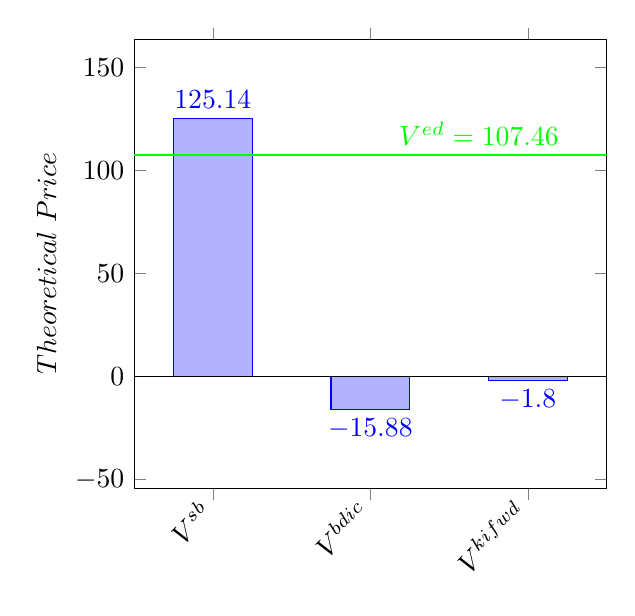
\begin{tikzpicture}
  \begin{axis}[
    enlargelimits=0.15,
    legend style={at={(0.5,-0.2)},
      anchor=north,legend columns=-1},
    ylabel={$Theoretical$ $Price$},
    symbolic x coords={Vsb,Vbdic,Vkifwd},
    xticklabels={$V^{sb}$, $V^{bdic}$, $V^{kifwd}$},
    xtick=data,
    nodes near coords,
    nodes near coords align={vertical},
    x tick label style={rotate=45,anchor=east},
    ybar=1pt,
    bar width=1cm,
    x=2cm,
    enlarge x limits={abs=1cm},
    enlarge y limits={abs=1cm},
    colormap/viridis
    ]
    \addplot coordinates {(Vsb,125.14) (Vbdic,-15.88)
        (Vkifwd,-1.80)};
    \draw [green] ({rel axis cs:0,0}|-{axis cs:Vsb,107.46}) -- ({rel axis cs:1,0}|-{axis cs:Vkifwd,107.46}) node [pos=0.73, above] {$V^{ed} = 107.46$};
        \draw [black] ({rel axis cs:0,0}|-{axis cs:Vsb,0}) -- ({rel axis cs:1,0}|-{axis cs:Vkifwd,0}) node [pos=0.73, above] {};
  \end{axis}
\end{tikzpicture}
\caption[CoCo price pursuant to the equity derivative approach and separation of its components]{CoCo price $V^{ed}$ and separation of its components under the equity derivative approach}
\label{pricecomponents}
\end{figure}

Thus, the price of the fictive CoCo $V^{ed}$ under the equity derivative approach is equal to 107.46. 

\section{Structural Approach} \label{sec:structuralapproach}
A third alternative to price CoCos is the structural approach of \citet{pennacchi2010structural}. The idea has its roots in the seminal work of \citet{merton1974pricing}, which aims to explain a company's default based on the relationship of its assets and liabilities under a standard Black-Scholes setting. \citet{pennacchi2010structural}'s approach expands the idea by modeling the stochastic evolution of a bank's balance sheet respectively of its components. In the following, the assets' rate of return process will be explained. Thereafter, we will outline the assumptions of the model regarding the various liabilities a bank issues to refinance itself including deposits, equity and coupon bonds in the form of CoCos. Lastly, a pricing formula will be illustrated.

\subsection{Structural Banking Model}
\subsubsection*{Bank Assets and Asset-To-Deposit Ratio}
\citet{pennacchi2010structural} assumes that a bank holds a portfolio of loans, equities and off-balance sheet positions as assets whose returns follow a jump-diffusion process. The change of this portfolio $A_t$ is determined by the rate of return and the cash in- respectively outflows. In this context, the symbol $*$ is used to point out the change in value of the portfolio which can be quantified by the rate of return, excluding net cashflows. The aforementioned instantaneous rate of return is denoted as $d A_t^*/ A_t^*$ and follows a stochastic process as stated below under the risk-neutral probability measure $\mathbb{Q}$:
\begin{align} \label{bankassetprocess}
\dfrac{d A_t^*}{A_t^*} &= \left( r_t - \lambda_t k_t \right) dt + \sigma dz + \left( Y_{q_{t^{-}}} -1\right) dq_t
\end{align}

It should be noted that $r_t$ stands for the risk-free interest rate as defined by the \citet{cox1985theory} term-structure model which will be discussed shortly. $dz$ is a Brownian motion, whereby $\sigma$ denotes the volatility of returns of the aforementioned asset portfolio. $q_t$ is a Poisson counting process which increases by one whenever a Poisson-distributed event respectively a jump occurs. Hence, the variable $dq_t$ is one whenever such a jump takes place and zero otherwise. The risk-neutral probability that a jump happens is equal to $\lambda_t dt$ where $\lambda_t$ stands for the intensity of the jump process. Variable $Y_{q_{t^{-}}}$ is a i.i.d. random variable drawn from $\ln(Y_{q_{t^{-}}}) \sim \Phi\left(\mu_{y}, \sigma^2_{y}\right)$ at time $t$ where $\mu_{y}$ stands for the mean jump size and $\sigma_{y}$ denotes the standard deviation of jumps. In case the random variable $Y_{q_{t^{-}}}$ is greater than one, an upward shift in the bank's asset value can be observed. If the value is smaller than one a downward jump takes place. Given that the risk-neutral expected proportional jump $k_t$ is defined as $k_t = E^\mathbb{Q}_t\left[ Y_{q_{t^{-}}} - 1 \right]$, one can determine $k_t$ with the following formula: $k_t = \exp(\mu_{y}+\dfrac{1}{2}\sigma_y^2) - 1$. Thus, the risk-neutral expected change in $A^*$ from the jump element $(Y_{q_{t^{-}}}-1)dq_t$ equals $\lambda_t k_t dt$ in $dt$. To sum up, the value development of a bank's asset portfolio $A_t^*$ follows largely a continuous process. But disruptive jumps may occur as illustrated below in the graph \ref{fig:jumpgraph}.\\
\begin{figure}[ht]
	\centering
	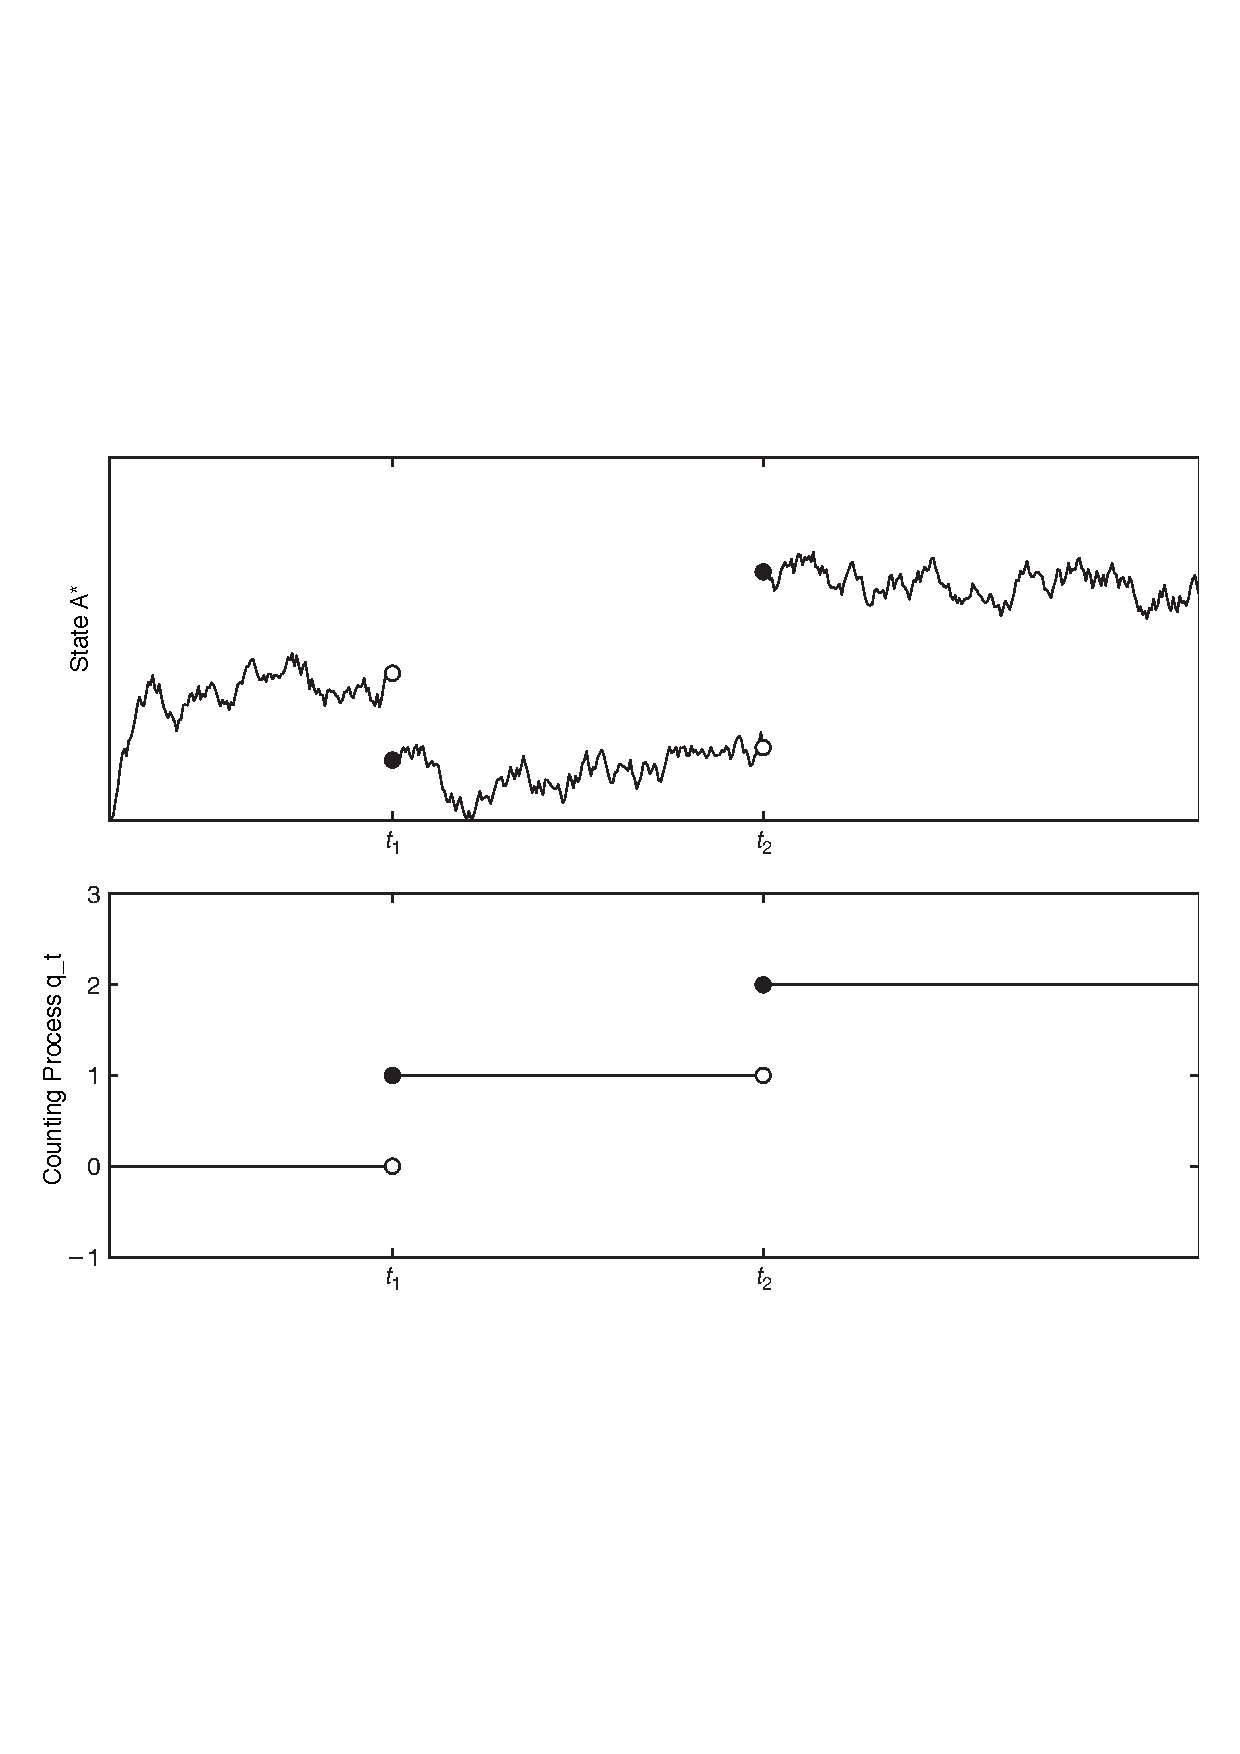
\includegraphics[trim=0.6cm 7.05cm 0.9cm 9cm, scale = 0.4]{media/jumpprocess} \par
	\caption[Jump-diffusion process]{The first graph shows two jumps in the state variable $A^*$ at discrete time points. Additionally, the corresponding Poisson counting process $q_t$ is highlighted in the second graph. \citep{ait2009handbook}}
	\label{fig:jumpgraph}
\end{figure}

The risk-neutral process of bank assets $A_t$ including the net cashflows is equal to the assets' rate of return less interest payments $r_t$ respectively premium payments $h_t$ to deposit holders proportionally to their deposits $D_t$. Furthermore, one has to subtract the coupon payments $c_t$ to CoCo investors proportionally to the face value $B$.
\begin{align} \label{bankassetprocess2}
dA_t &= \left[ \left( r_t - \lambda k \right) A_t - \left( r_t + h_t \right) D_t - c_t B \right] dt + \sigma A_t dz + \left( Y_{q_{t^{-}}} - 1 \right) A_t dq
\end{align}

By substituting variable $x_t$ with $A_t/D_t$ and anticipating the deposit growth process $g\left(x_t - \hat{x}\right)$ as pointed out by equation \ref{depositgrowthprocess}, the risk neutral process of the asset-to-deposit ratio equals:
\begin{align}
\dfrac{dx_t}{x_t}&= \dfrac{dA_t}{A_t} - \dfrac{dD_t}{D_t}\\ \nonumber
&= \left[ \left(r_t - \lambda k \right) - \dfrac{r_t + h_t + c_t b_t}{x_t} - g\left(x_t - \hat{x}\right)\right] dt + \sigma dz + \left( Y_{q_{t^{-}}} - 1 \right) dq_t
\end{align}

with
\begin{align}
b_t &= \dfrac{B}{D_t}
\end{align}

Lastly, an application of It\^{o}'s lemma for jump-diffusion processes leads to the following formula for the asset-to-deposit ratio process:
\begin{align}
d \ln\left(x_t\right) &= \left[ \left( r_t - \lambda k \right) - \dfrac{r_t + h_t + c_t b_t}{x_t} - g\left( x_t - \hat{x} \right) - \dfrac{1}{2} \sigma^2 \right] dt \\ \nonumber
&+ \sigma dz + \ln Y_{q_{t^{-}}} dq_t
\end{align}

\subsubsection*{Default-Free Term Structure}
\label{termstructure}

\citet{pennacchi2010structural} applies the term-structure specifications of \citet{cox1985theory} to model the risk-neutral process of the instantaneous risk-free interest rate $dr_t$ which is defined as follows:
\begin{align}
dr_t = \kappa \left(\bar{r} - r_t \right) dt + \sigma_r \sqrt{r_t} d \zeta
\end{align}

Note that $\kappa$ is the speed of convergence, $\bar{r}$ is the long-run equilibrium interest rate, $r_t$ is the continuous short-term interest rate, $\sigma_r$ is the instantaneous volatility and $d\zeta$ is a Brownian motion.\\

A zero bond can be priced using the \citet{cox1985theory} specifications under the no-arbitrage assumption. This implies that the price of a risk-free zero bond at time t that pays the amount of $1$ currency unit in $\tau = T - t$ is given by:
\begin{align} \label{zerobondprice}
P\left( r_t, \tau \right) = A\left(\tau \right) \exp\left[ - B\left( \tau \right) r_t \right]
\end{align}

with
\begin{align}
A\left( \tau \right) &= \left\{ \dfrac{2\theta \exp{\left[ \left(\theta + \kappa \right) \dfrac{\tau}{2}\right] } }{ \left( \theta + \kappa \right) \left[ \exp\left( \theta \tau \right) - 1 \right] +2 \theta} \right\}^{2 \kappa \bar{r} / \sigma_r^2 }\nonumber
\end{align}

\begin{align}
B\left(\tau \right) &= \dfrac{2 \left[ \exp\left( \theta \tau \right) -1 \right]}{\left( \theta + \kappa \right) \left[ \exp\left( \theta \tau \right) -1 \right] +2\theta } \nonumber
\end{align}

\begin{align}
\theta = \sqrt{\kappa^2 + 2 \sigma_r^2}\nonumber
\end{align}

The cost of replication of a risk-free coupon bond that pays a continuous coupon of $c_r dt$ is equal to a set of zero bonds which can be priced with equation \ref{zerobondprice}. Therefore, the fair coupon rate $c_r $ of such a coupon bond at time $t$, which is issued at par, equals:
\begin{align}
c_r &= \dfrac{1-A\left( \tau \right) \exp\left[ - B\left( \tau \right) r_t \right]}{\int_0^{\tau} A \left( s \right) \exp\left[ -B\left(s\right) r_t \right] ds}\nonumber \\
&\approx \dfrac{1- A\left( \tau \right)\exp\left[ -B \left( \tau \right) r_t \right]}{\sum_{i=1}^{i=n} A\left( \Delta t \times i \right) \exp\left[ -B \left( \Delta t \times i \right) r_t \right] \Delta t}
\end{align}

with
\begin{align}
n &= \dfrac{\tau}{\Delta t}
\end{align}

\subsubsection*{Deposits and Insurance Premium}
Bank deposits are not riskless because depositors may suffer losses if a bank's asset value $A_t$ is worth less than the deposits $D_t$. That said, one can assume that a bank is closed by the deposit insurer when the asset-to-deposit ratio $x_t$ is less or equal to one. A bank might become distressed due to continuous downward movements in its asset value. Then, the bank will be shut down with $A_{t_{b}}=D_t$ and subsequently, depositors will not face any loss. However, depositors may experience severe losses when a downward jump in asset value happens at a discrete point in time, $\hat{t}$. It may be that the downward jump in asset value exceeds the bank's capital. If such a jump occurs the instantaneous proportional loss to deposits will equal $\left(D_t - Y_{q_{t^{-}}} A_{\hat{t^{-}}}  \right) / D_t$.\\

The fair deposit insurance premium $h_t$ for deposit holders can be derived with equation \ref{insurancepremium}. The equation illustrates that $h_t$ is closely related to the asset-to-deposit ratio $x_t$:
\begin{align} \label{insurancepremium}
 h_t &=  \lambda \left[ \Phi\left( -d_1 \right) - x_{t^{-}} \exp\left( \mu_y + \dfrac{1}{2} \sigma_y^2 \right) \Phi\left( -d_2 \right)    \right]
\end{align}
with
\begin{align}
d_1 &= \dfrac{\ln\left( x_{t^{-}}\right) + \mu_y}{\sigma_y}\\
d_2 &= d_1 + \sigma_y
\end{align}

The model assumes that a bank pays continuously a total interest and deposit premium of $\left( r_t + h_t \right) D_t dt$ to each depositor. Hence, one might recognize that the deposits change only because of comparatively higher deposit inflows than outflows. Empirical research of \citet{adrian2010liquidity} suggests that banks have a target capital ratio and that deposit growth is positively related to the current asset-to deposit ratio:
\begin{align}\label{depositgrowthprocess}
\dfrac{dD_t}{D_t} &= g\left(x_t -\hat{x} \right)dt
\end{align}

$\hat{x} > 1$ is a bank's target asset-to-deposit ratio with $g$ being a positive constant. Whenever the actual asset-to-deposit ratio is higher than its target, $x_t > \hat{x}$, a bank will shrink its balance sheet. Thus, the deposit growth rate $g\left( x_t - \hat{x} \right)$ in the time interval $dt$, leads to a mean-reverting tendency for the asset-to-deposit ratio $x_t$.

\subsubsection*{Equity and Conversion Threshold}

As stated originally, the conversion of a CoCo at time $t_c$ occurs when the asset-to-deposit ratio $x_{t_c}$ meets the trigger level $\bar{x}_{t_c}$. The conversion threshold can also be expressed relative to the original equity-to-deposits ratio $\bar{e}$. This is favourable because the equity value is directly observable in the market whereas the asset value is not. The relationship between the equity threshold $\bar{e}$ and the asset-to-deposit threshold $\bar{x}_{t_c}$ can be summarized as follows:
\begin{align}
\bar{e} &= \dfrac{E_{t_c}}{D_{t_c}} = \dfrac{A_{t_c} - D_{t_c} - pB}{D_{t_c}} = \bar{x}_{t_c} - 1 - p b_{t_c}
\end{align}

Hence, it is possible to specify exactly the conversion trigger of a CoCo bond. This will be important for the valuation part.

\subsubsection*{CoCos}
The valuation of a CoCo can be accomplished with a Monte Carlo simulation of both the asset and the deposit process. Along the asset-to-deposit ratio process, the CoCo pays coupons and the nominal at maturity unless the CoCo has not been triggered. If the trigger event occurs the conversion amount is paid out. \citep{wilkens2014contingent} The price of the CoCo $V^{st}$ is equal to the risk-neutral expectation of the aforementioned cashflows as derived by \citet{pennacchi2010structural}:
\begin{align}
V_0^{st} &= E_0^{\mathbb{Q}} \left[ \int_0^T \exp\left(-\int_0^t r_s ds\right) v\left( t \right) dt \right]
\end{align}

Please note $v(t)$ stands for a coupon payment at date $t$ which equals $c_t B$ as long as the CoCo has not been triggered. If the CoCo does not convert until maturity $T$, a final payout of $B$ will be performed. However, if the CoCo triggers early at time $t_c$, there is the one-time cashflow of $pB$. Parameter $p$ determines the maximum conversion amount of new equity per par value of contingent capital. Thereafter, $v(t)$ is zero.

\subsection{Parameter Classification and Adjustment}
The biggest challenge of the structural approach is the accurate estimation of its input parameters. A reliable estimation is not straightforward as most of the variables are not directly observable in the market. \citep{de2014handbook} A complete overview of all input variables is presented in table \ref{tbl:structuralapproachdata}.\\ 

In general, one can distinguish three parameter types. The first group comprises parameters which are directly observable in the market respectively in a CoCo's term sheet. The second category encompasses variables that are linked to a bank's balance sheet or strategy and are thus semi-observable. Finally, the third group covers parameters which are in fact not observable and are determined based on expert judgement or calibration to market data. \citep{wilkens2014contingent} Hereinafter, major input variables and their adjustment will be described.

\begin{table}
	\setlength{\extrarowheight}{2.5pt}
	\centering
	\footnotesize
	\begin{tabular}{p{1.8cm}p{6.8cm}p{2.4cm}p{2.5cm}}
		\toprule
			 & \textbf{Description} & \textbf{Usage} & \textbf{Source} \\
		\midrule
			$T$ & Maturity & Static input & Term sheet\\
			$B$ & Notional & Static input & Term sheet \\
			$c$ & Coupon rate & Static input & Term sheet\\ 
			$p$ & Conversion factor & Static input & \\
			$\,\,\,$$\hookrightarrow$ $S^*$ & Trigger share price & Static input & Term sheet\\
			$\,\,\,$$\hookrightarrow$ $C_p$ & Conversion price & Static input & Term sheet\\
			$x_t$ & Asset-to-deposit ratio & Dynamic input & \\
			$\,\,\,$$\hookrightarrow$ $S_t$ & Share price & Dynamic input & Market data\\
			$\,\,\,$$\hookrightarrow$ $n_t$ & Number of shares & Dynamic input & Market data\\
			$\,\,\,$$\hookrightarrow$ $D_t$ & Deposit value & Dynamic input & Balance sheet\\
			$\hat{x}$ & Target asset-to-deposit ratio & Static input & \\
			$\,\,\,$$\hookrightarrow$ $A_\text{Target}$ & Target asset value & Static input & Term sheet \\
			$\,\,\,$$\hookrightarrow$ $D_\text{Target}$ & Target deposit value & Static input & Term sheet\\
			$g$ & Mean-reversion speed & Static input & Expert judgm.  \\
			$\sigma_A$ & Annual asset return volatility & Dynamic input & \\
			$\,\,\,$$\hookrightarrow$ $D_t$ & Deposit value & Dynamic input & Balance sheet\\
			$\,\,\,$$\hookrightarrow$ $S_t$ & Share price & Dynamic input & Market data\\
			$\,\,\,$$\hookrightarrow$ $n_t$ & Number of shares & Dynamic input & Market data\\
			$\,\,\,$$\hookrightarrow$ $\sigma_E$& Historic share price volatility & Static input & Market data\\
			$\,\,\,$$\hookrightarrow$ $r_t$ & Risk-free interest rate & Dynamic input & Market data \\
			$\lambda$ & Jump intensity in asset return process & Static input  & Expert judgm.  \\	
			$\mu_y$ & Mean jump size in asset return process & Static input &  \\
			$\sigma_y$ & Jump volatility in asset return process & Static input &  \\
			$\,\,\,$$\hookrightarrow$ $S_\text{past}$ &  Historic share price data & Static input & Market data\\
			$r_t$ & Risk-free interest rate & Dynamic input & Market data \\
			$\bar{r}$ & Long-term risk-free interest rate & Static input & \\
			$\sigma_r$ &Interest rate volatility & Static input & \\
			$\kappa$ & Speed of convergence & Static input & \\
			$\,\,\,$$\hookrightarrow$ $r_\text{past}$ & Set of historic risk-free interest rate data & Static input & Market data\\
			$\rho$ & Correlation between Brownian motion for asset returns and interest rate process  & Static input & \\ 
			$\,\,\,$$\hookrightarrow$ $S_\text{past}$ &  Historic share price data & Static input & Market data\\
			$\,\,\,$$\hookrightarrow$ $r_\text{past}$ &  Historic risk-free interest rate data & Static input & Market data\\
			$\bar{e}$ & Conversion threshold of the market value of original shareholders' equity to deposit value & Static input & \\
			$\,\,\,$$\hookrightarrow$ $S^*$ & Trigger share price & Static input & Term sheet\\
			$\,\,\,$$\hookrightarrow$ $n_0$ & Initial number of shares & Static input & Term sheet\\
			$\,\,\,$$\hookrightarrow$ $D_0$ & Initial deposit value & Static input & Term sheet\\
			$b_0$ & Ratio of the contingent capital's nominal to the initial value of deposits & Dynamic input & \\
			$\,\,\,$$\hookrightarrow$ $D_t$ & Initial deposit value & Dynamic input & Balance sheet \\
			$\,\,\,$$\hookrightarrow$ $B$ & Contingent capital nominal & Static input & Term sheet\\
		\bottomrule
	\end{tabular}
	\caption[Parameter classification of the structural approach]{Parameter classification of the structural approach}
	\label{tbl:structuralapproachdata}
\end{table}

\subsubsection*{Bank Assets and Asset-To-Deposit Ratio}
The structural approach models the development of the asset-to-deposit ratio $x_t$ over time. On this account, the paper attempts to obtain $x_t$ with equity and deposit estimates. The equity component is equivalent to the daily observable market capitalization $S_t n_t$. Moreover, deposit values are inferred from a bank's quarterly published balance sheet data while assuming that all liabilities are deposits. The deposit level $D_t$ is interpolated between the disclosure of financial statements. \citep{wilkens2014contingent} Hence one can determine the asset-to-deposit ratio with the following equation: $x_t = (S_t n_t + D_t)/D_t$. Furthermore, the target asset-to-deposit ratio $\hat{x}$ is driven by the strategy of the issuing bank and can be described as follows: $\hat{x} = A_\text{Target}/D_\text{Target}$.\\

The asset volatility $\sigma_A$ is also an important input variable of the asset process but is not observable on a daily basis. Therefore, the paper evaluates the asset volatility based on its relation to the share price volatility $\sigma_E$ as described by \citet{merton1974pricing}. The source code can be found in section \ref{estimateMertonParameter}. Moreover, the structural model assumes that asset returns follow a jump-diffusion process. This implies that the probability of extreme asset returns is larger than predicted by normally distributed asset returns. To estimate the parameters that govern the distribution of the jump size, the paper assumes that historical share price returns are a reliable proxy for asset jumps. The mean jump size $\mu_y$ and the jump volatility $\sigma_y$ are estimated based on threshold exceedance methods and assumptions on the jump intensity $\lambda$, which is in turn used to specify the number of exceedances over a threshold. \citep{longin2001extreme} The implementation is presented in section C.1.3.

\subsubsection*{Default-Free Term Structure}
For the \citet{cox1985theory} model pricing parameters are estimated with the approach of \citet{remillard2013statistical}. The approach calibrates the long-term risk-free interest rate $\bar{r}$, the interest rate volatility $\sigma_r$ and the speed of convergence $\kappa$. To do so, maximum likelihood techniques for dependent observations are applied. The approach takes a series of daily sovereign bond yields as input which have maturities of one, three, six and twelve months. The implementation of this approach can be found in section \ref{estimateCIRParameter}. Additionally, the correlation between the geometric Brownian motion for asset returns and the interest rate process $\rho$ is approximated with the five year daily correlation between a sovereign bond of the same tenure respectively denomination and a related stock market index.

\subsubsection*{Deposits and Insurance Premium}
A reasonable mean-reversion speed $g$ for deposits is assumed to be equal to 0.5. The assumption follows the assessment of \citet{pennacchi2010structural}. He argues that this estimate for $g$ gives a plausible deposit's half time of around 3 years. The deposit's half-time in turn describes the time it takes for the deposit value to move half the distance towards its target value.

\subsubsection*{Equity and Conversion Threshold}
Similar to the credit and equity derivative approach the conversion factor $p$ depends on the trigger share price $S^*$ and the conversion price $C_p$: $p = S^*/C_p$. Moreover, the conversion threshold $\bar{e}$ of a CoCo also relies on the trigger share price $S^*$ as outlined by $\bar{e} = E_\text{Trigger}/D_0 = n S^*/D_0$.

\subsection{Model Application}
The parameters shown in table \ref{tbl:playa} serve to price a generic CoCo pursuant to the structural approach. The pricing results can be found in figure \ref{fig:comparison}.
\begin{figure}[H]
\centering
\begin{tikzpicture}
\begin{axis}[width=11cm, height=11cm, axis y line*=left, ylabel={$Theoretical$ $Price$}, ymin =70,
        ylabel near ticks, xlabel={$Number$ $of$ $Paths$ $per$ $Simulation$}, xlabel near ticks, cycle list={blue}, yticklabel=\pgfmathparse{\tick}\pgfmathprintnumber{\pgfmathresult}\,\ , scale only axis=false, boxplot/draw direction=y,xtick={1,2,3,4,5,6,7,8},xticklabels={1,5,10,50,100,500,1000,5000}]
 \addplot+[boxplot prepared={
        lower whisker=80.45, lower quartile=89.74,
        median=97.67, upper quartile=114.35,
        upper whisker=137.52}] coordinates {};
    \addplot+[boxplot prepared={
        lower whisker=83.98, lower quartile=94.98,
        median=98.22, upper quartile=104.26,
        upper whisker=119.47}] coordinates {};
    \addplot+[boxplot prepared={
        lower whisker=89.43, lower quartile=94.08,
        median=97.30, upper quartile=101.62,
        upper whisker=108.38}] coordinates {};
    \addplot+[boxplot prepared={
        lower whisker=93.12, lower quartile=96.16,
        median=97.55, upper quartile=99.06,
        upper whisker=102.19}] coordinates {};
    \addplot+[boxplot prepared={
        lower whisker=94.98, lower quartile=96.82,
        median=97.78, upper quartile=98.50,
        upper whisker=102.02}] coordinates {};
    \addplot+[boxplot prepared={
        lower whisker=95.93, lower quartile=97.17,
        median=97.71, upper quartile=98.05,
        upper whisker=99.32}] coordinates {};
      \addplot+[boxplot prepared={
        lower whisker=97.06, lower quartile=97.57,
        median=97.80, upper quartile=98.09,
        upper whisker=98.72}] coordinates {};
    \addplot+[boxplot prepared={
        lower whisker=97.27, lower quartile=97.60,
        median=97.77, upper quartile=97.93,
        upper whisker=98.48}] coordinates {};
     \addplot [green, mark = x, mark size = 0.25cm] coordinates {( 1, 70.1)};
     \addplot [green, mark = x, mark size = 0.25cm] coordinates {( 2, 70.3)};
     \addplot [green, mark = x, mark size = 0.25cm] coordinates {( 3, 70.6)};
     \addplot [green, mark = x, mark size = 0.25cm] coordinates {( 4, 71.1)};
     \addplot [green, mark = x, mark size = 0.25cm] coordinates {( 5, 72)};
     \addplot [green, mark = x, mark size = 0.25cm] coordinates {( 6, 74)};
     \addplot [green, mark = x, mark size = 0.25cm] coordinates {( 7, 80)};
     \addplot [green, mark = x, mark size = 0.25cm] coordinates {( 8, 145)};
      \draw [yellow] ({rel axis cs:0,0}|-{axis cs:0,107.46}) -- ({rel axis cs:1,0}|-{axis cs:9,107.46}) node [pos=0.73, below] {$V^{ed} = 107.46$};
      \draw [yellow] ({rel axis cs:0,0}|-{axis cs:0,111.31}) -- ({rel axis cs:1,0}|-{axis cs:9,111.31}) node [pos=0.73, above] {$V^{cd} = 111.31$};
\end{axis}
\begin{axis}[
	width=11cm, height=11cm,
	xtick={1,2,3,4,5,6,7,8}, xticklabels={1,5,10,50,100,500,1000,5000},
        %scale only axis=false,
        hide x axis,
        axis y line*=right,
        ylabel={$Average$ $Time$ $per$ $Simulation$ $in$ $Seconds$},
        ylabel near ticks,
        %ymin = 0, ymax = 10,
        ytick={1,2,3,4,5,6,7,8,9}, yticklabels={0,100,200,300,400,500,600,700,800}
    ]
    %\addplot [green, mark = x, mark size = 0.25cm] coordinates {( 8, 7)}
\end{axis}
%      \addplot [black, mark = *] coordinates {( 1, 1600)};
\end{tikzpicture}
\caption[Comparison of pricing results]{Comparison of pricing results}
\label{fig:comparison}
\end{figure}

Running the monte-carlo simulation with different path numbers per simulation leads to a broad range of prices. As shown by the blue whisker plots one can directly see the minimum, the 25\%-percentile, the median, the 75\%-percentile and the maximum for each path number. One hundred simulations have been conducted for each boxplot. It becomes apparent that the price stability is tightly connected to the average time per simulation as shown by the green crosses. For 5000 paths per simulation one can derive a median price of $V^{sa}$ of $97.77$. The derived value is significantly lower than those of the credit derivative approach $V^{cd}$ and the equity derivative approach $V^{ed}$ which are highlighted in yellow. This might be the case due to the fact that the structural approach accounts for discontinuous returns.


%\begin{table}[H]
%	\setlength{\extrarowheight}{2.5pt}
%	\centering
%	\footnotesize
%	\begin{tabular}{lrp{10cm}}
%		\toprule
%			 & \textbf{Value} & \textbf{Comment} \\
%		\midrule
%			$T$ & $10$yrs & Maturity \\
%			$B$ & $100.00\%$ & Notional \\
%			$c$ & $6.00\%$ & Coupon rate \\
%			$S_0$ & 120 & Initial share price\\
%			$n_0$ & 1 & Initial number of shares\\
%			$S^*$ & 60 & Trigger share price\\
%			$C_p$ & 75 & Conversion price\\
%			$g$ & $10$ & Mean-reversion speed \\
%			$\lambda$ & $2$& Jump intensity in asset return process\\			
%			$\mu_y$ &$0$ & Mean jump size in asset return process\\
%			$\sigma_y$ &$20\%$ & Jump volatility in asset return process\\		
%			$r_0$ & $1.00 \%$ & Initial Risk-free interest rate\\
%			$\bar{r}$ & $ 6.00\%$ & Long-term risk-free interest rate\\
%			$\sigma_r$ & $5.00\%$ & Interest rate volatility \\
%			$\kappa$ & $4.00\%$ & Speed of convergence \\
%			$\rho$ & $50\%$ & Correlation between Brownian motion for asset returns and interest rate process\\
%			$\sigma_E$& 30\% & Historic share price volatility\\
%			$D_0$ & 880 & Initial deposit value \\
%			$A_\text{Target}$ & 1015 & Target asset value\\
%			$D_\text{Target}$ & 883.05 & Target deposit value\\
%			$CC$ & 30 & Contingent capital value \\
%		\bottomrule
%	\end{tabular}
%	\caption[Parameter specification of structural approach application]{Parameter specification of structural approach application \citep{erismann2015pricing}}
%	\label{tbl:playa}
%\end{table}

\begin{table}[H]
	\setlength{\extrarowheight}{2.5pt}
	\centering
	\footnotesize
	\begin{tabular}{lrp{10cm}}
		\toprule
			 & \textbf{Value} & \textbf{Comment} \\
		\midrule
			$T$ & $10$yrs & Maturity \\
			$B$ & $100.00\%$ & Notional \\
			$c$ & $6.00\%$ & Coupon rate \\
			$p$ & $0.8$ & Conversion factor\\
			$\,\,\,$$\hookrightarrow$ $S^*$ & 60 & Trigger share price\\
			$\,\,\,$$\hookrightarrow$ $C_p$ & 75 & Conversion price\\
			$x_0$ & $1.1364$ & Initial asset-to-deposit ratio\\
			$\,\,\,$$\hookrightarrow$ $S_0$ & 120 & Initial share price\\
			$\,\,\,$$\hookrightarrow$ $n$ & 1 & Number of shares\\
			$\,\,\,$$\hookrightarrow$ $D_0$ & 880 & Initial deposit value \\
			$\hat{x}$ & $1.12$ & Target asset-to-deposit ratio\\
			$\,\,\,$$\hookrightarrow$ $A_\text{Target}$ & 1000 & Target asset value\\
			$\,\,\,$$\hookrightarrow$ $D_\text{Target}$ & 892.86 & Target deposit value\\
			$g$ & $10$ & Mean-reversion speed \\
			$\sigma_A$ & $3.63\%$ & Asset volatility \\
			$\,\,\,$$\hookrightarrow$ $D_0$ & 880 & Initial deposit value\\
			$\,\,\,$$\hookrightarrow$ $n$ & 1 & Number of shares \\
			$\,\,\,$$\hookrightarrow$ $S_0$ & 120 & Initial share price\\
			$\,\,\,$$\hookrightarrow$ $\sigma_E$& 30\% & Historic share price volatility\\
			$\,\,\,$$\hookrightarrow$ $r_0$ & $3.00\%$ & Initial risk-free interest rate\\
			$\lambda$ & $2$& Jump intensity in asset return process\\			
			$\mu_y$ &$0$ & Mean jump size in asset return process\\
			$\sigma_y$ &$2.00\%$ & Jump volatility in asset return process\\
			$\,\,\,$$\hookrightarrow$ $S_\text{past}$ &  & Historic share price data\\		
			$r_0$ & $3.00 \%$ & Risk-free interest rate\\
			$\bar{r}$ & $ 6.00\%$ & Long-term risk-free interest rate\\
			$\sigma_r$ & $5.00\%$ & Interest rate volatility \\
			$\kappa$ & $4.00\%$ & Speed of convergence \\
			$\,\,\,$$\hookrightarrow$ $r_\text{past}$ &  & Set of historic risk-free interest rate data \\
			$\rho$ & $50\%$ & Correlation between Brownian motion for asset returns and interest rate process\\
			$\,\,\,$$\hookrightarrow$ $S_\text{past}$ &  & Historic share price data \\
			$\,\,\,$$\hookrightarrow$ $r_\text{past}$ &  & Historic risk-free interest rate data \\
			$\bar{e}$ & $6.81\%$ & Conversion threshold of the market value of shareholders' equity to original deposit value\\
			$\,\,\,$$\hookrightarrow$ $S^*$ & 60 & Trigger share price\\
			$\,\,\,$$\hookrightarrow$ $n$ & 1 & Number of shares\\
			$\,\,\,$$\hookrightarrow$ $D_0$ & 880 & Initial deposit value \\
			$b_0$ & $3.41\%$ & Ratio of contingent capital's nominal to the initial deposit value\\
			$\,\,\,$$\hookrightarrow$ $D_0$ & 880 & Initial deposit value \\
			$\,\,\,$$\hookrightarrow$ $CC$ & 30 & Contingent capital value \\
		\bottomrule
	\end{tabular}
	\caption[Parameter specification of structural approach application]{Parameter specification of structural approach application}
	\label{tbl:playa}
\end{table}




